% Copyright (C) 2005-2015 Airbus - EDF - IMACS - Phimeca
% Permission is granted to copy, distribute and/or modify this document
% under the terms of the GNU Free Documentation License, Version 1.2
% or any later version published by the Free Software Foundation;
% with no Invariant Sections, no Front-Cover Texts, and no Back-Cover
% Texts.  A copy of the license is included in the section entitled "GNU
% Free Documentation License".
\renewcommand{\etapemethodo}{B}
\renewcommand{\nomfichier}{docref_B201_Graph}
\renewcommand{\titrefiche}{Using QQ-plot to compare two samples}

\Header

\MathematicalDescription{

  \underline{\textbf{Goal}} \vspace{2mm}

  Let $X$ be a scalar uncertain variable modelled as a random variable. This method deals with the construction of a dataset prior to the choice of a probability distribution for $X$. A QQ-plot (where "QQ" stands for "quantile-quantile") is a tool that may be used to compare two samples $\left\{x_1,\ldots,x_N \right\}$ and $\left\{x'_1,\ldots,x'_M \right\}$; the goal is to determine graphically whether these two samples come from the same probability distribution or not. If this is the case, the two samples should be aggregated in order to increase the robustness of further statistical analyses.

  \vspace{2mm}

  \underline{\textbf{Principle of the method}} \vspace{2mm}

  A QQ-plot is based on the notion of quantile. The $\alpha$-quantile $q_{X}(\alpha)$ of $X$, where $\alpha \in (0, 1)$, is defined as follows:
  \begin{align*}
    \Prob{ X \leq q_{X}(\alpha)} = \alpha
  \end{align*}
  If a sample $\left\{x_1,\ldots,x_N \right\}$ of $X$ is available, the quantile can be estimated empirically:
  \begin{enumerate}
  \item the sample $\left\{x_1,\ldots,x_N \right\}$ is first placed in ascending order, which gives the sample $\left\{ x_{(1)},\ldots,x_{(N)} \right\}$;
  \item then, an estimate of the $\alpha$-quantile is:
    \begin{align*}
      \widehat{q}_{X}(\alpha) = x_{([N\alpha]+1)}
    \end{align*}
    where $[N\alpha]$ denotes the integral part of $N\alpha$.
  \end{enumerate}

  Thus, the $j^\textrm{th}$ smallest value of the sample $x_{(j)}$ is an estimate $\widehat{q}_{X}(\alpha)$ of the $\alpha$-quantile where $\alpha = (j-1)/N$ ($1 < j \leq N$). Let us then consider our second sample $\left\{x'_1,\ldots,x'_M \right\}$; this one also provides an estimate $\widehat{q}'_{X}(\alpha)$ of this same quantile:
  \begin{align*}
    \widehat{q}'_{X}(\alpha) = x'_{([M\times(j-1)/N]+1)}
  \end{align*}
  If the the two samples correspond to the same probability distribution, then $\widehat{q}_{X}(\alpha)$ and $\widehat{q}'_{X}(\alpha)$ should be close. Thus, graphically, the points $\left\{ \left( \widehat{q}_{X}(\alpha),\widehat{q}'_{X}(\alpha)\right),\  \alpha = (j-1)/N,\ 1 < j \leq N \right\}$ should be close to the diagonal.

  The following figure illustrates the principle of a QQ-plot with two samples of size $M=50$ and $N=50$. Note that the unit of the two axis is that of the variable $X$ studied. In this example, the points remain close to the diagonal and the hypothesis "the two samples come frome the same distribution" does not seem irrelevant, even if a more quantitative analysis (see \otref{docref_B202_Smirnov}{Smirnov test}) should be carried out to confirm this.

  \begin{center}
    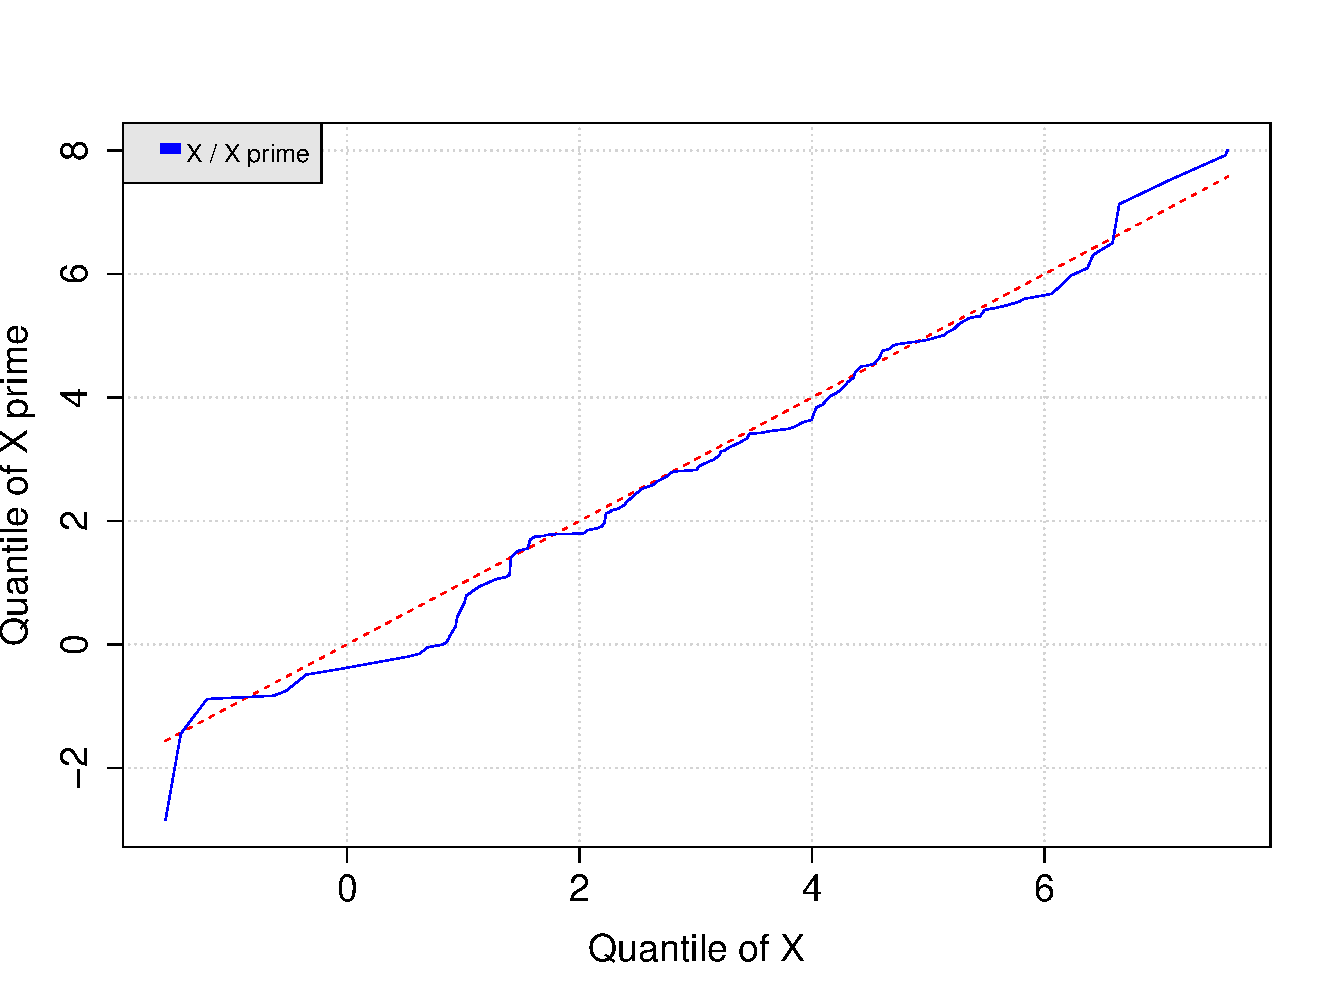
\includegraphics[scale=0.5]{Figures/QQplotOk.pdf}
  \end{center}

  In this second example, the two samples clearly arise from two different distributions.

  \begin{center}
    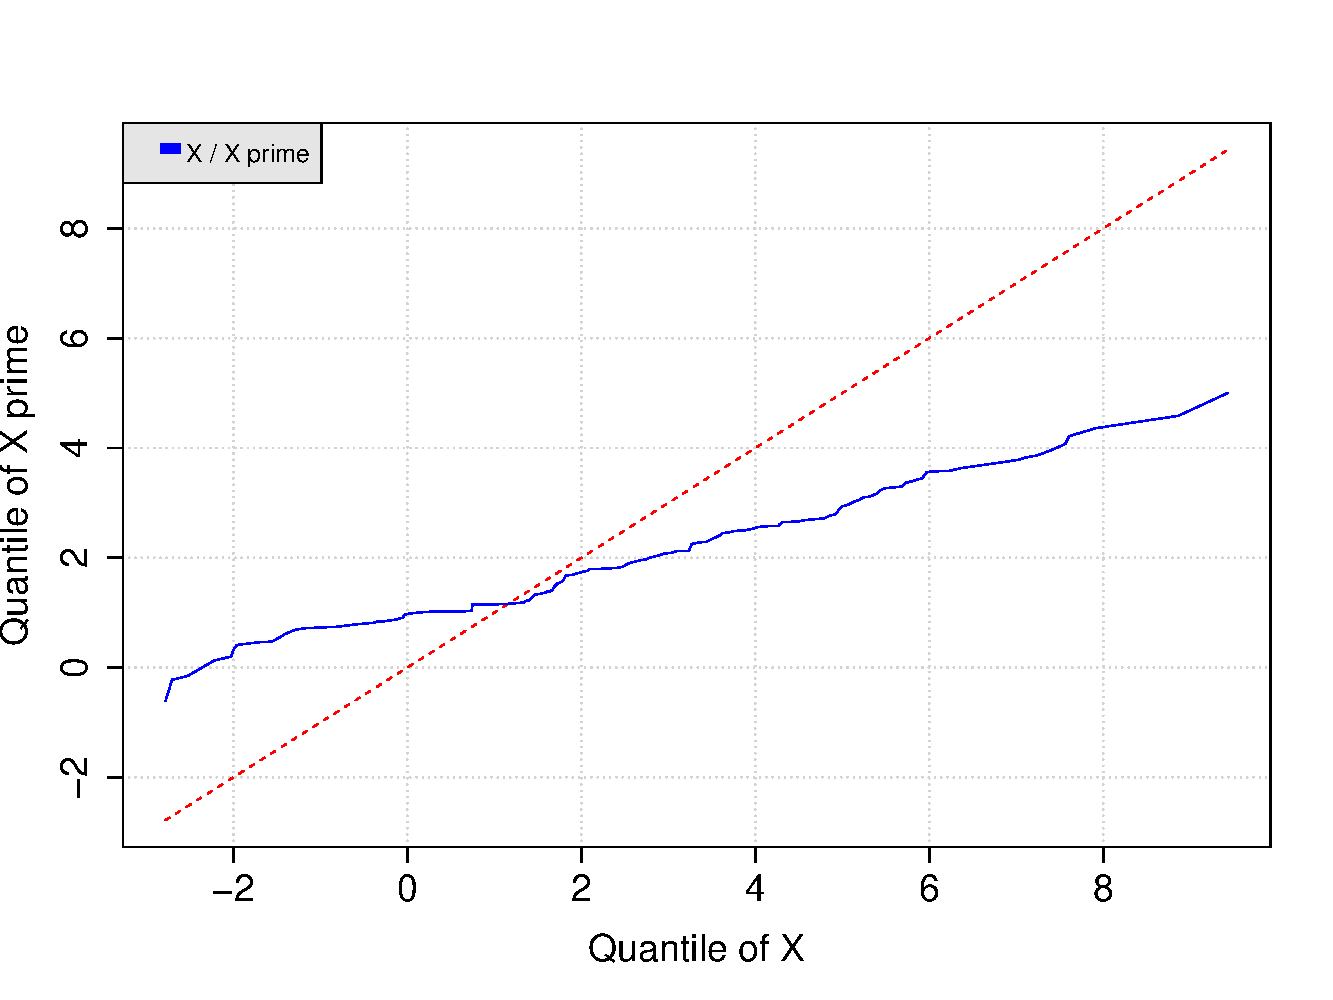
\includegraphics[scale=0.5]{Figures/QQplotBad.pdf}
  \end{center}

  \vspace{2mm}
}
{
}

\Methodology{
  This method is used in step B "Quantifying Sources of Uncertainty". It is a tool for the construction of a dataset that can be used afterwards to choose  a probability distribution for some uncertain variables defined in step A "Specifying Criteria and the Case Study".
}
            {
              A QQ-plot is a graphical analysis, the conclusion of which remains obviously subjective. The reader is referred to \otref{docref_B202_Smirnov}{Smirnov test} for a more quantitative analysis.
              % Bibliography
              The following bibliographical references provide main starting points for further study of this method:
              \begin{itemize}
              \item Saporta, G. (1990). "Probabilités, Analyse de données et Statistique", Technip
              \item Dixon, W.J. \& Massey, F.J. (1983) "Introduction to statistical analysis (4th ed.)", McGraw-Hill
                % \item NIST/SEMATECH e-Handbook of Statistical Methods, http://www.itl.nist.gov/div898/handbook/
              \item D'Agostino, R.B. and Stephens, M.A. (1986). "Goodness-of-Fit Techniques", Marcel Dekker, Inc., New York.
              \item Bhattacharyya, G.K., and R.A. Johnson, (1997). "Statistical Concepts and Methods", John Wiley and Sons, New York.
              \item Sprent, P., and Smeeton, N.C. (2001). "Applied Nonparametric Statistical Methods -- Third edition", Chapman \& Hall
            \end{itemize}}
